\setcounter{section}{2}

\Needspace{5\baselineskip}
\hypertarget{ux6d41ux5f62ux5047ux8bbeux4e0eux8d85ux8fdeux63a5}{%
\section{流形假设与超连接}\label{ux6d41ux5f62ux5047ux8bbeux4e0eux8d85ux8fdeux63a5}}

\Needspace{5\baselineskip}
\hypertarget{ux4e00ux6d41ux5f62ux5047ux8bbe}{%
\subsection{一、流形假设}\label{ux4e00ux6d41ux5f62ux5047ux8bbe}}

虽然数据嵌入在一个高维的欧氏空间中，但有意义的数据分布实际上集中在一个维数低得多的低维流形上。也就意味着，对于一个神经网络（或其局部块），从输入x到输出y之间经过的变换是低维的，y-x是分布在低维空间内的向量。

Yoshua Bengio团队在论文《Representation Learning: A Review and New Perspectives》中指出，深度神经网络之所以能泛化，是因为它们成功地学习到了数据所在的低维流形结构，并将其``展开''到了平坦的特征空间中。

\Needspace{5\baselineskip}
\hypertarget{ux4e8cux8d85ux8fdeux63a5hyper-connectionshc}{%
\subsection{二、超连接（Hyper Connections，HC）}\label{ux4e8cux8d85ux8fdeux63a5hyper-connectionshc}}

\Needspace{5\baselineskip}
\hypertarget{ux4e00ux6269ux5c55ux6b8bux5deeux6d41ux5bbdux5ea6}{%
\subsubsection{（一）扩展残差流宽度}\label{ux4e00ux6269ux5c55ux6b8bux5deeux6d41ux5bbdux5ea6}}

在传统的残差神经网络中，y=f(x)+x，f(x)是神经网络主体函数。这里f(x)的输入和输出维度均和x、y的维度相同，均为d\_model。但实际上，f(x)的有效维度应该远小于x、y的表征维度，因此传统的残差神经网络x与y之间的``信息高速公路''太窄，``损失''了很多x、y的有效表征维度，还容易引起网络训练不稳定。

为此，HC将残差流的维度（信息传输维度）和网络主体函数f的维度（计算维度）解耦，加大了残差流的维度，并引入可学习的降维矩阵Hl\_pre和升维矩阵Hl\_post，完成残差流维度和计算维度之间的转换，从而在不显著增大总参数量的前提下，显著增大实际能承载的信息量。

\begin{figure}[htbp]
\centering
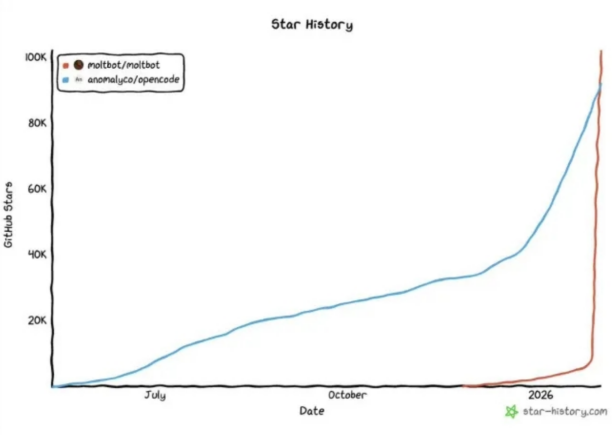
\includegraphics{images/image-0033.png}
\caption{残差连接与超连接结构对比图}
\end{figure}

\Needspace{5\baselineskip}
\hypertarget{ux4e8cux5f15ux5165ux53efux5b66ux4e60ux7684ux6b8bux5deeux8fdeux63a5ux77e9ux9635}{%
\subsubsection{（二）引入可学习的残差连接矩阵}\label{ux4e8cux5f15ux5165ux53efux5b66ux4e60ux7684ux6b8bux5deeux8fdeux63a5ux77e9ux9635}}

\Needspace{5\baselineskip}
从理论上讲，前面的做法已经比较完备了。但HC还引入了残差连接矩阵Hl\_res，对残差流进行线性变换。原因：

\begin{enumerate}
\def\labelenumi{\arabic{enumi}.}
\item
  更好地拟合弯曲流形：深度神经网络由多层构成，对于任意的l，第l层的输出x\_l+1和输入x\_l之差确实都分布在低维空间中，但每一层对应的低维空间的取向往往有一定差异，现实中它们构成的整体流形在高维空间中往往是弯曲的。引入可学习的残差连接矩阵可以让函数的高维空间基底向量灵活地旋转（即不同维度之间可以发生信息交换），增强拟合弯曲流形的性能。
\item
  引入遗忘机制：早期的特征（比如第一层的边缘纹理）在第100层可能已经完全没用了，变成了噪音，但如果不引入Hl\_res，它很难被去除，只能被后面的层通过LayerNorm强行压制，这会浪费宝贵的动态范围。当Hl\_res的特征值小于1时，它起到了遗忘机制的作用。
\end{enumerate}

\Needspace{5\baselineskip}
\hypertarget{ux4e09ux6d41ux5f62ux7ea6ux675fux8d85ux8fdeux63a5}{%
\subsection{三、流形约束超连接}\label{ux4e09ux6d41ux5f62ux7ea6ux675fux8d85ux8fdeux63a5}}

流形约束超连接（Manifold-Constrained Hyper-Connections，mHC）由 DeepSeek 团队于 2025 年首次公开，是对 HC 的重要工程化改进。

\Needspace{5\baselineskip}
\hypertarget{ux4e00hcux5b58ux5728ux7684ux95eeux9898}{%
\subsubsection{（一）HC存在的问题}\label{ux4e00hcux5b58ux5728ux7684ux95eeux9898}}

\begin{enumerate}
\def\labelenumi{\arabic{enumi}.}
\item
  数值不稳定：原始的HC中，连接矩阵没有额外的约束，信号在经过多层传播后容易发生梯度爆炸（可达到数百甚至上千倍）或梯度消失，且这还破坏了恒等映射的特性。
\item
  显存和通信开销大：通道变宽意味着显存读写（I/O）和通信成本大幅度增加，即``显存墙''问题。
\end{enumerate}

\Needspace{5\baselineskip}
\hypertarget{ux4e8cmhcux7684ux6539ux8fdb}{%
\subsubsection{（二）mHC的改进}\label{ux4e8cmhcux7684ux6539ux8fdb}}

mHC将变换Hl\_res，Hl\_pre和Hl\_post均限制在了特定的流形上。

\Needspace{4\baselineskip}
\begin{enumerate}
\def\labelenumi{\arabic{enumi}.}
\tightlist
\item
  将Hl\_res限制为双拟随机矩阵
\end{enumerate}

利用Sinkhorn-Knopp 算子，将Hl\_res限制为各元素非负、每行和为1、每列和为1的双拟随机矩阵。本质上说，双拟随机矩阵是排列矩阵的凸组合（排列矩阵：每行、每列只有一个1，其他均为0，一个矩阵乘以排列矩阵，等价于将原矩阵的特征维度向量交换位置），在几何上也就意味着``对于输入向量进行多种旋转（加权）''。它的重复应用会单调地增加跨流的特征融合和信息混合。

\Needspace{5\baselineskip}
此外，该方法在工程上还有两方面优点：

（1）其2-范数有界且不超过1，学习到的映射是非扩张的，可有效缓解梯度爆炸问题。

（2）双拟随机矩阵集对矩阵乘法具有封闭性，确保了跨多层的复合残差映射仍保持双拟随机，从而可在整个模型深度上维持稳定性。

\begin{figure}[htbp]
\centering
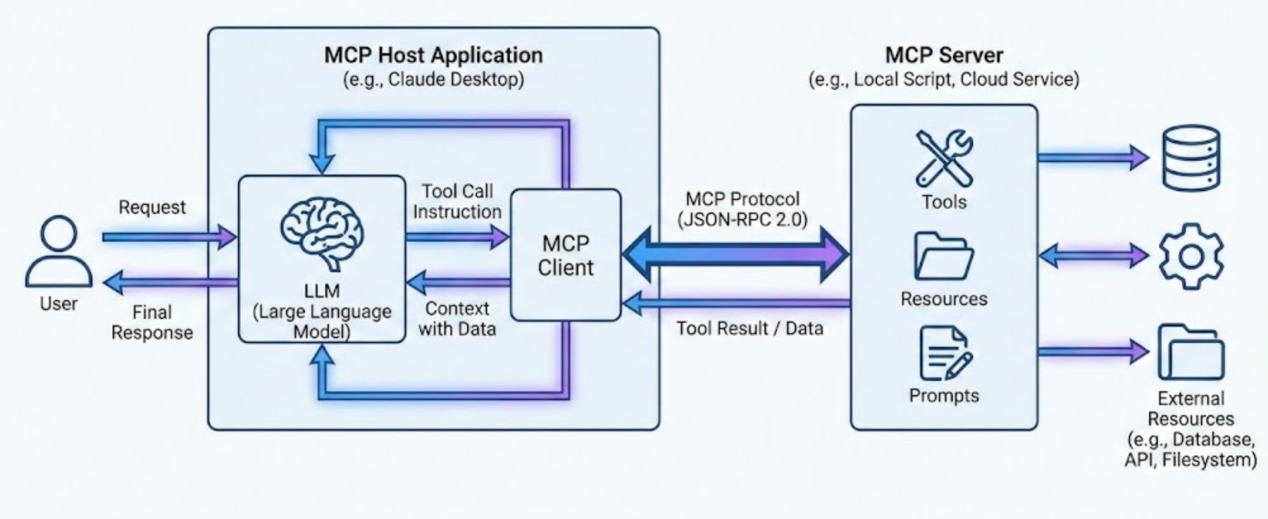
\includegraphics{images/image-0034.png}
\caption{残差连接、超连接与流形约束超连接结构对比图}
\end{figure}

\Needspace{4\baselineskip}
\begin{enumerate}
\def\labelenumi{\arabic{enumi}.}
\setcounter{enumi}{1}
\tightlist
\item
  对Hl\_pre和Hl\_post施加非负约束
\end{enumerate}

Hl\_pre是一个特征重组矩阵，调节各个特征的信号。其第i行第j列的值代表：用于本层计算的低维特征中的第i个维度中，来自高维特征中第j个维度的权重。mHC对两个矩阵均用sigmoid函数转换以保证非负性，提高稳定性，避免正负参数抵消。

注意：这里不用Softmax，因为Softmax要求每行权重之和为1。Hl\_pre如果为10000*1000维，则Softmax会导致输入总信号减小10倍（单个维度信号大小数量级不变，维度除以10）。作为一个门控机制的实现模块，这是不可接受的。

\FloatBarrier
\Needspace{5\baselineskip}
\hypertarget{ux53c2ux8003ux6587ux732e-103}{%
\subsection{参考文献}\label{ux53c2ux8003ux6587ux732e-103}}

\vspace{0.25em}
\begin{itemize}
\tightlist
\item
  Bengio, Y., Courville, A., \& Vincent, P. (2013). \href{https://arxiv.org/abs/1206.5538}{Representation Learning: A Review and New Perspectives}. IEEE Transactions on Pattern Analysis and Machine Intelligence, 35(8), 1798-1828.
\item
  Zhu, D., et al.~(2025). \href{https://arxiv.org/abs/2409.19606}{Hyper-Connections}. arXiv:2409.19606.
\item
  Xie, Z., Wei, Y., Cao, H., et al.~(2025). \href{https://arxiv.org/abs/2512.24880}{mHC: Manifold-Constrained Hyper-Connections}. arXiv:2512.24880.
\end{itemize}

\clearpage
